This work consists in solving the two main problems of "k-means"-like 
algorithms described in Section \ref{related} and \ref{problem_definition}:
choosing the $k$ parameter and placing the $k$ initial centroids.
The only assumption is that the dataset is generated from one or more gaussian
disitributions.


\subsection*{The choice of $k$}
The most common scenario does not involve a domain expert. In this way there is 
no prior knowledge that can be used to guess a proper and reasonable value for $k$.
The main idea behind the solution proposed in this work is that of exploiting density
analysis to get an initial estimate of the number of clusters in the data.

More formally, a \emph{peak detection} procedure is used to retrieve 
all the local maxima in the density function for each feature\footnote{This is equivalent to
finding all the local maxima in the density functions for each axis, if the item considered is
a point in an n-dimensional euclidean space.} of the items in the dataset. In this way,
a peak is defined as a data sample that is either larger than its two neighboring samples.
This results in a list of peaks for each feature space and finally a n-dimensional grid
matching every possible peack among all the features available is created
(see Algorithm \ref{alg:grid_creation}).
\begin{algorithm}[h]
 \KwIn{xs, points'x values}
 \KwIn{ys, points'y values}
 \KwResult{array, initial centroids}

 hx = computeMarginalDensity (xs)\;
 hy = computeMarginalDensity (ys)\;

 px = detectPeaks (hx)\;
 py = detectPeaks (hy)\;

 centroids = []\;
 \For{i $\in$ px}{
    \For{j $\in$ py}{
        centroids += (hx.x[i], hy.x[j])\;
    }
 }
% return [(hx[x], hy[y]) for x in px for y in py]
 \KwRet{centroids}
 \caption{Initial centroids identification}\label{alg:grid_creation}
\end{algorithm}


As it is possible to notice from Figure~\ref{grid}, the black diamonds on the top and on
the left sub-figures are the peaks found on the density distribution function among all
the points in the dataset, the orange points in the central sub-figure represent the
grid of all the potential centroids.
In this way, the worst-case scenario is taken into account, allowing this approach not
to miss any potential centroid in the whole dataset\footnote{This approach produces an 
over-estimation of the real number of centroids, including also possible false-negatives.}.

\begin{figure*}
  \center{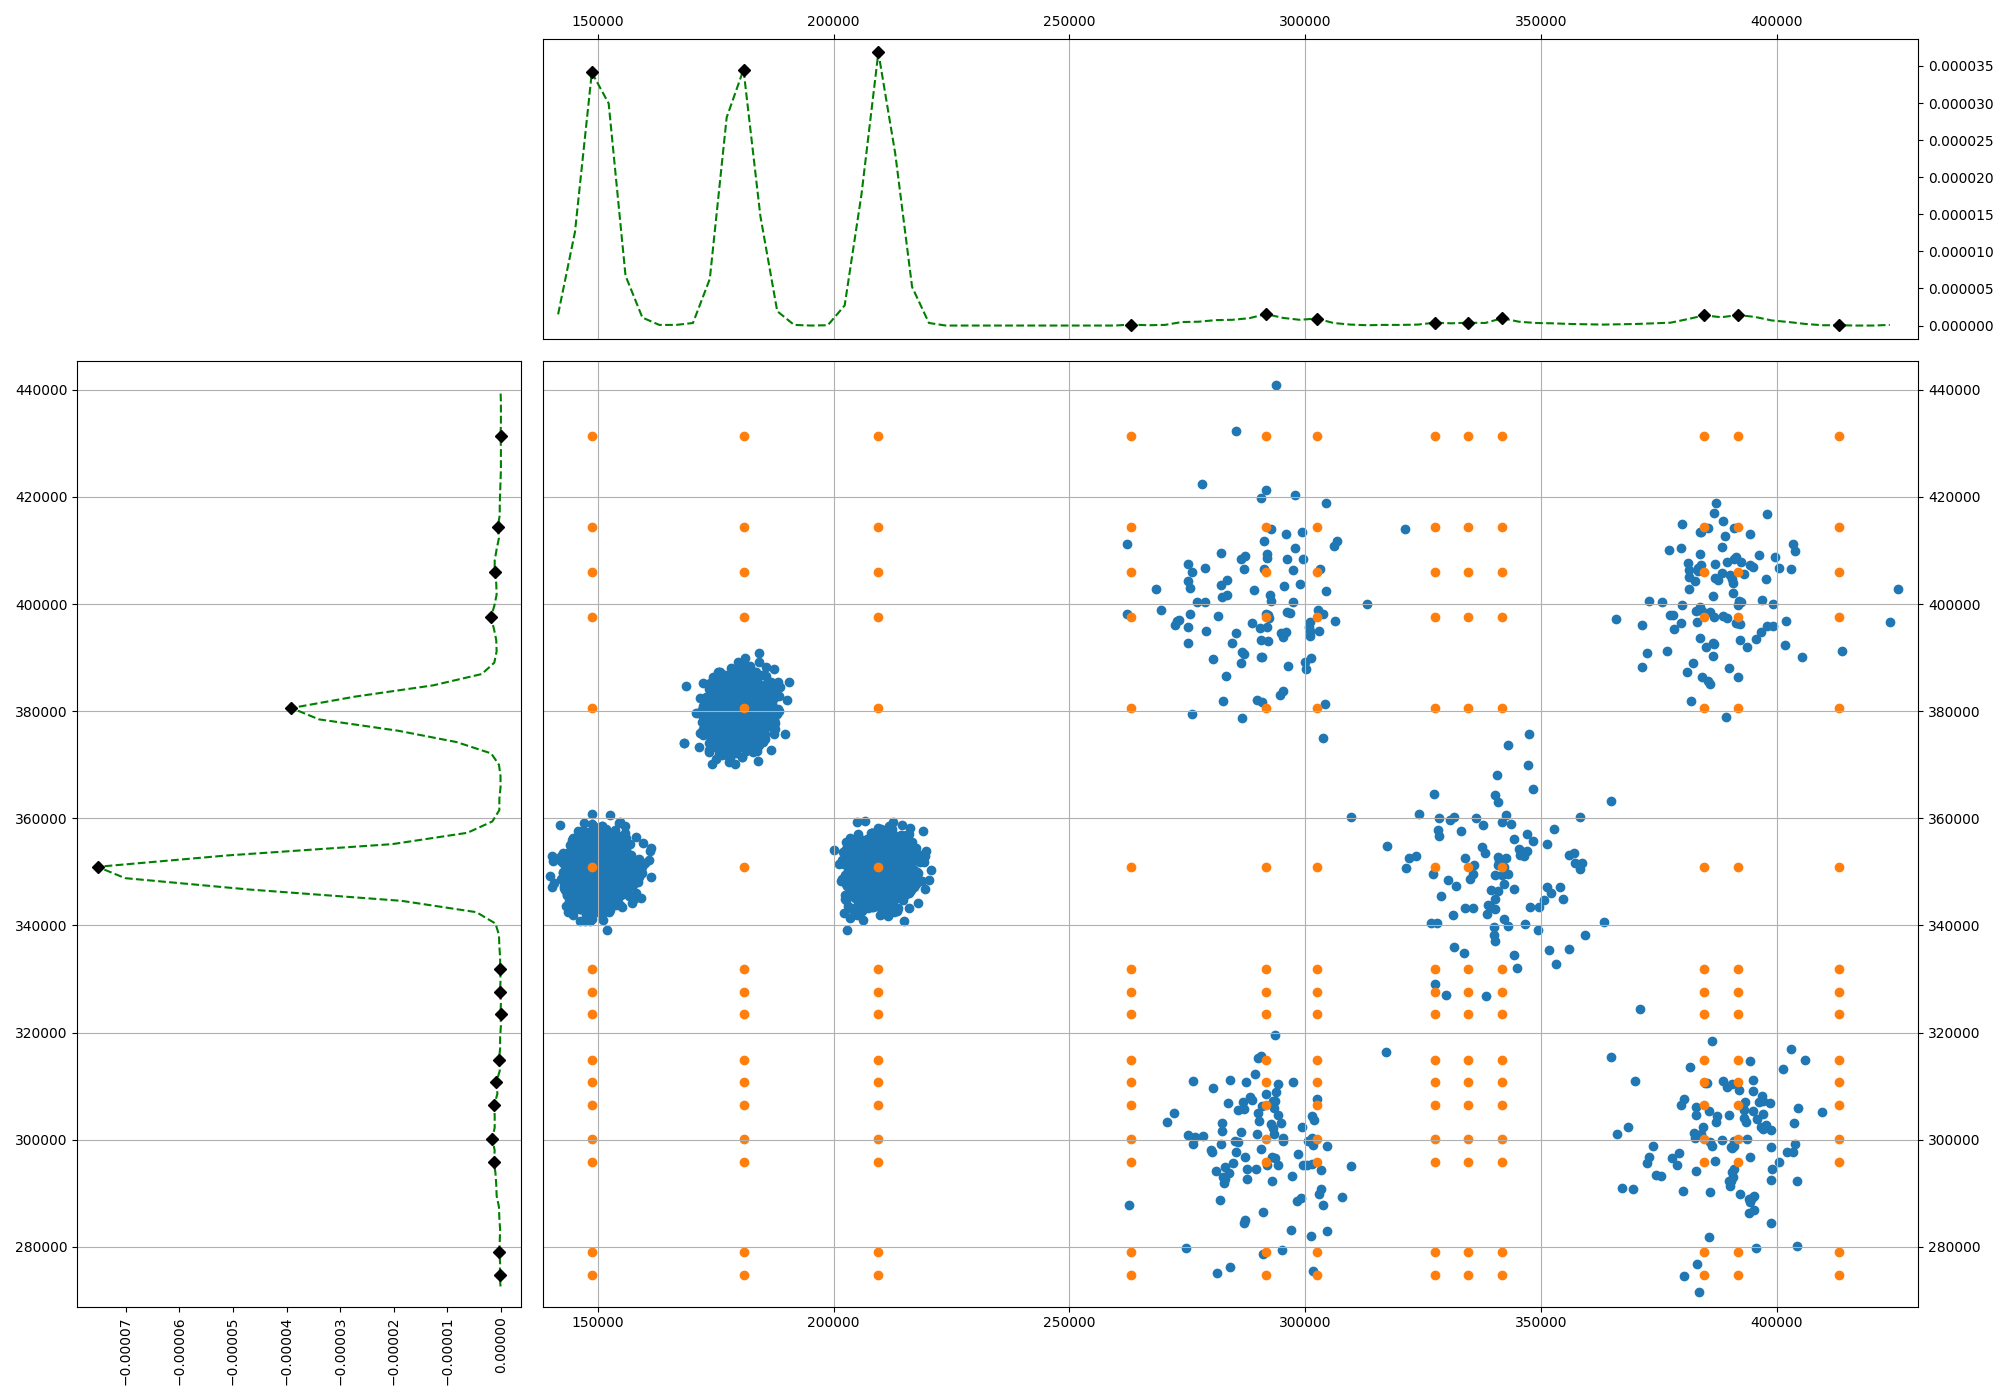
\includegraphics[width=0.7\textwidth]{unbalance_rescaled_coolfig.png}}
  \caption{The grid with all the potential centroids computed from the peaks.}
  \label{grid}
\end{figure*}

Moreover, among all the potential peaks created, only those which have at least one data
item assigned after a run of the k-means are kept. This allows to discard all the 
false-positives that were found creating all the possible touples in all the feature spaces.
Furthermore, it represents the refinement step for the algorithm.

Finally, the number of items in this grid represents the value for the $k$ parameter.


\subsection*{Centroids bootstrap}
The other important phase is to find a good positioning of the $k$ initial centroids.
The main idea behind this feature proceeds as follows:
\begin{enumerate}
    \item \label{step1} use the peak location as the one of the centroids.
    \item build an ellipse around every centroid with the $(a,b)$ parameters (namely the x-axis
        and the y-axis radius) applying the formula in Equation \ref{ellipse_params} (see
        Algorithm~\ref{alg:find_ellipses}).
    \item merge all the ellipses that intersect with each other (see 
        Algorithm~\ref{alg:merge_procedure}).
    \item go to \ref{step1} until convergence or some other exit criterion is met.
\end{enumerate}

\begin{algorithm}[h]
    \KwIn{centroids, [(centroidId,x,y)]}
    \KwIn{clusters, [\{id: [(x, y)]\}]}
    \KwResult{ellipses}

    cDesnity = {}\;
    $dx$ = $dy$ = []\;
    \For{cluster $\in$ clusters}{
        $(x_{\mu}, x_{\sigma})$ = normFit (cluster.x)\;
        $(y_{\mu}, y_{\sigma})$ = normFit (cluster.y)\;

        $dx$ += px = normPDF $(x_{\mu}, x_{\mu}, x_{\sigma})$\;
        $dy$ += py = normPDF $(y_{\mu}, y_{\mu}, y_{\sigma})$\;

        cDensity[cluster.id] = $((x_{\mu}, x_{\sigma}, px), (y_{\mu}, y_{\sigma}, py))$\;
    }

    ellipses = []\;
    \For{$(c, ((x_x, x_y, x_p), (y_x, y_y, y_p))) \in$ cDensity}{
        ellipses += $(c$,\\
            $((x_x, x_y, (x_p - dx_{\mu})/dx_{\sigma})$, \\
            $(y_x, y_y,  (y_p - dy_{\mu})/dy_{\sigma})))$\;
    }

    \KwRet{ellipses}
    \caption{Compute Estimated Influence Area}\label{alg:find_ellipses}
\end{algorithm}

\begin{algorithm}[h]
    \KwIn{ellipses}
    \KwIn{cstats, \{id: (xsum, ysum, n)\}}
    \KwResult{centroids}

~\\
    // Fing merges
    merges = []
    \For{$e_0, e_1 \in ellipses$}{
        // Compute $a,b$ ellipse paramteres (Eq~\ref{ellipse_params})\\
        $eia_0$ = computeEIA ($e_0$)\;
        $eia_1$ = computeEIA ($e_1$)\;

        \If{$Ellipse(e_0, eia_0) \cap Ellipse(e_1, eia_1) \neq \varnothing$}{
            merges += $(e_0, e_1)$\;
        }
    }

~\\
    // Apply merges
    merged = {}\;
    \For{($e_0, e_1) \in merges$}{
        $e_0$ = findCurrentIdIfMerged ($e_0$, merged)\;
        $e_1$ = findCurrentIdIfMerged ($e_1$, merged)\;

        $(xsum_0, ysum_0, n_0)$ = cstats[$e_0$.id]\;
        $(xsum_1, ysum_1, n_1)$ = cstats[$e_1$.id]\;

        cstats[$e_0$.id] = \\
            $(xsum_0 + xsum_1, ysum_0 + ysum_1, n_0 + n_1)$\;
        merged[$e_1$.id] = $e_0$.id\;
    }

~\\
    // Derive centroids
    centroids = []\;
    \For{(c, (xsum, ysum, n)) $\in$ cstats}{
        centroids += $(xsum/n, ysum/n)$\;
    }

    \KwRet{centroids}
    \caption{Merge centroids with overlapping EIA}\label{alg:merge_procedure}
\end{algorithm}


The formula (Equation~\ref{ellipse_params}) to compute the heigth and the width of the ellipses 
is the key aspect of the proposed merging strategy.
\begin{equation}
\label{ellipse_params}
    f(std, cdens) = ((std * 2 * 0.35) + (cdens * 0.7)) * 5
\end{equation}
Where:
\begin{itemize}
    \item $std$ is the standard deviation of the gaussian distribution underlying the cluster
    \item $cdens$ is the value of the gaussian distribution Probability Distribution Function (PDF)
        in the mean.
\end{itemize}

The reasoning behing the formula works as follows. Given the mean and the standard deviation ($std$)
of a cluster, $std$ is doubled to take both the sides of the gaussian distribution into account.
The 0.35 and the 0.7 values allows the density in the mean value of the gaussian distribution ($cdens$) 
to influence more the size of the ellipse rather than its standard deviation ($std$). Finally, 5 is
an overall scaling factor useful to allow the comparison of cluster with very different densities.

From an higher point of view, Equation \ref{ellipse_params} represents the \emph{estimated influence area} 
for every cluster. As the name suggests, this depicts (also visually) the area of influence a cluster
has on all the others.\\
As it is possible to see from Figure~\ref{start}, the ellipses represent all the initial
\emph{estimated influence areas} starting from all the potential centroids after discarding
all the centroids that has no item belonging to it (which are clearly false-positives).
If two clusters' estimated influence area has a non-empty intersection, this
means that they can be collapsed and become a single bigger cluster.\\
The Figures~\ref{start}, \ref{middle} and \ref{end} depicts the trend and the position of the
\emph{estimated influence areas} during an example merging procedure.

Moreover, as it is possible to notice from Figure \ref{end}, the approach described in this
section successfully started with many potential centroids (see Figure~\ref{start}) and, after a
few iterations, converged and found the 8 clusters in the dataset (see Figure~\ref{end}). 

\begin{figure}[t]
  \center{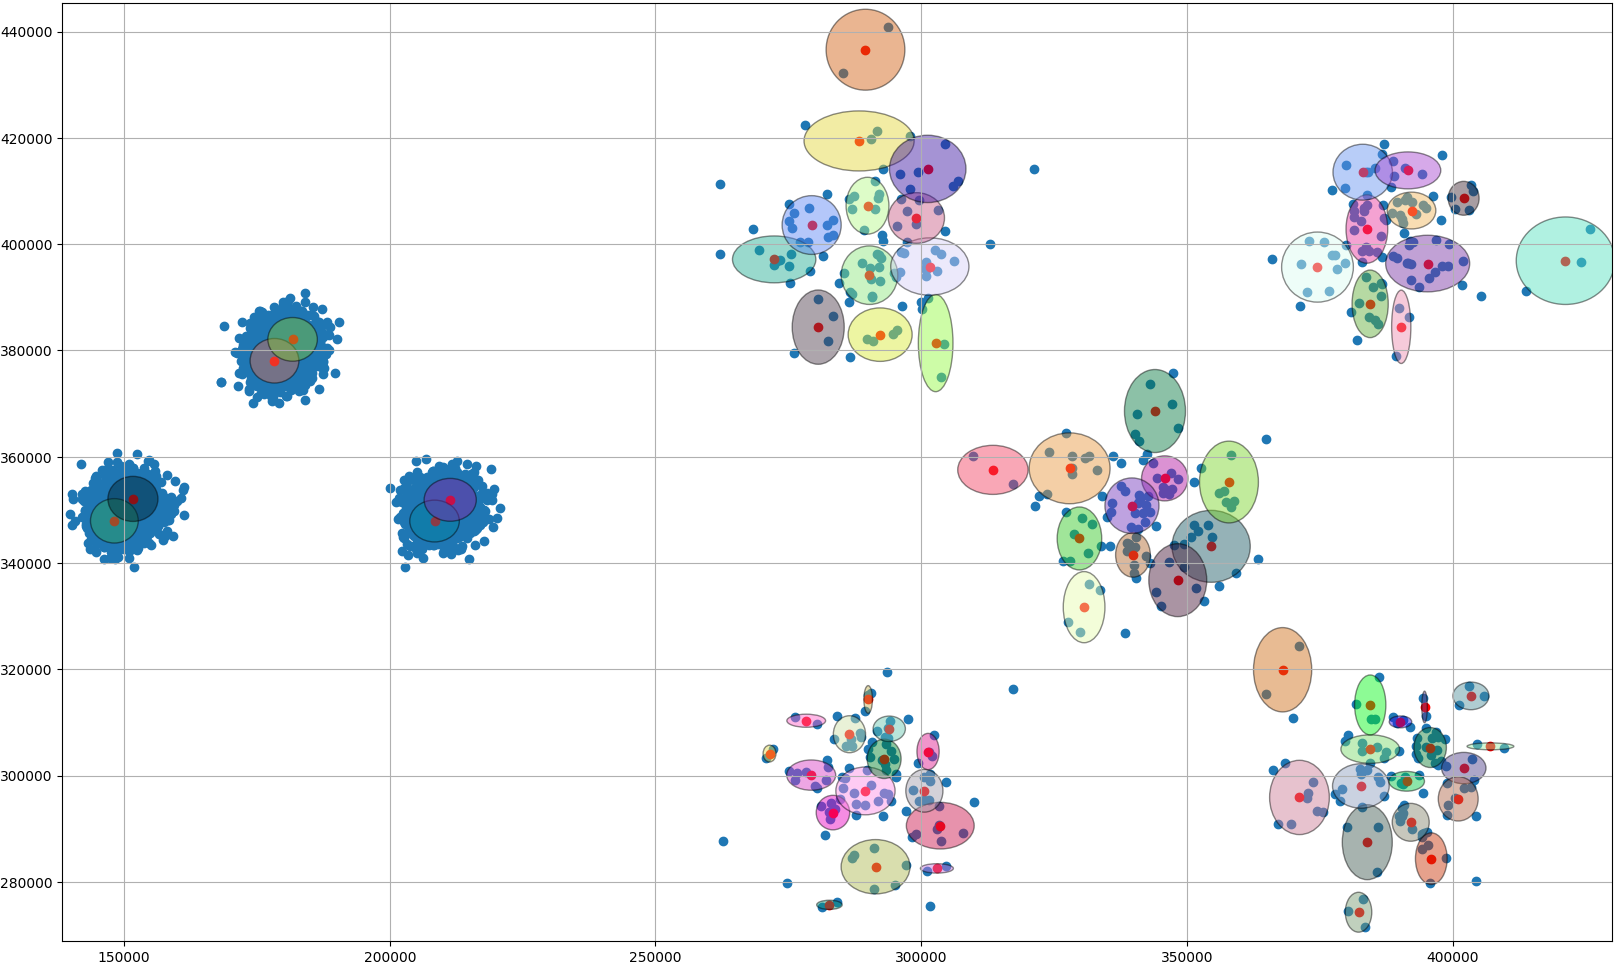
\includegraphics[width=0.5\textwidth]{unbalance_rescaled_density_0.png}}
  \caption{The first estimated influence areas after filtering some of the false-positives.}
  \label{start}
\end{figure}

\begin{figure}[t]
  \center{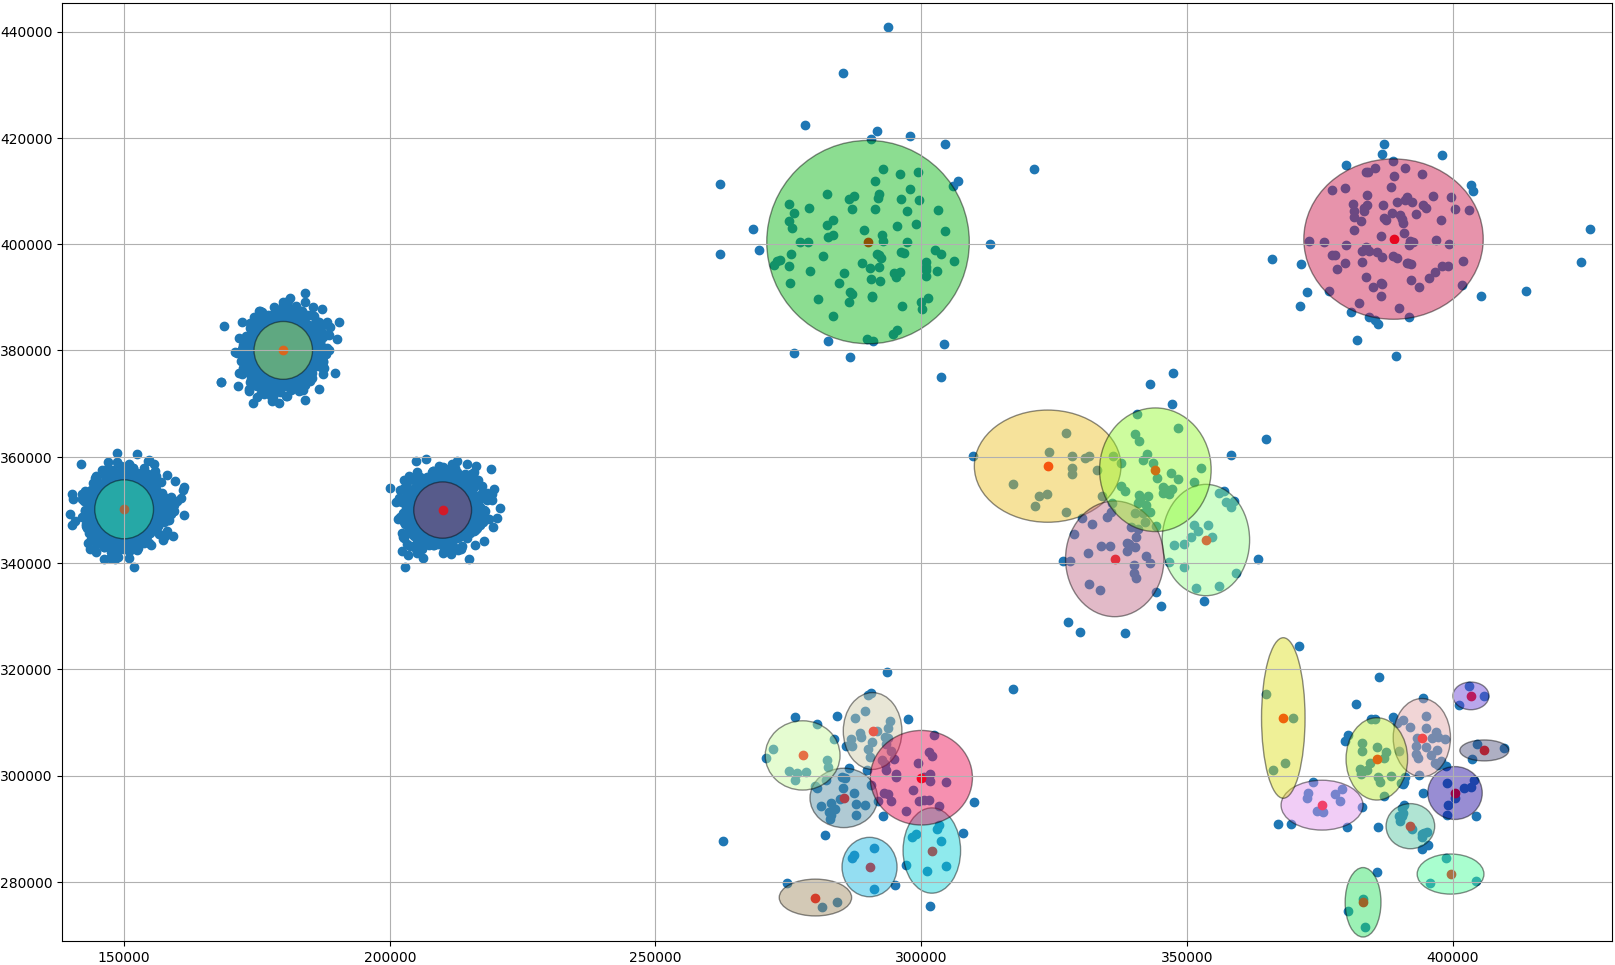
\includegraphics[width=0.5\textwidth]{unbalance_rescaled_density_3.png}}
  \caption{The situation after 4 iterations.}
  \label{middle}
\end{figure}

\begin{figure}[t]
  \center{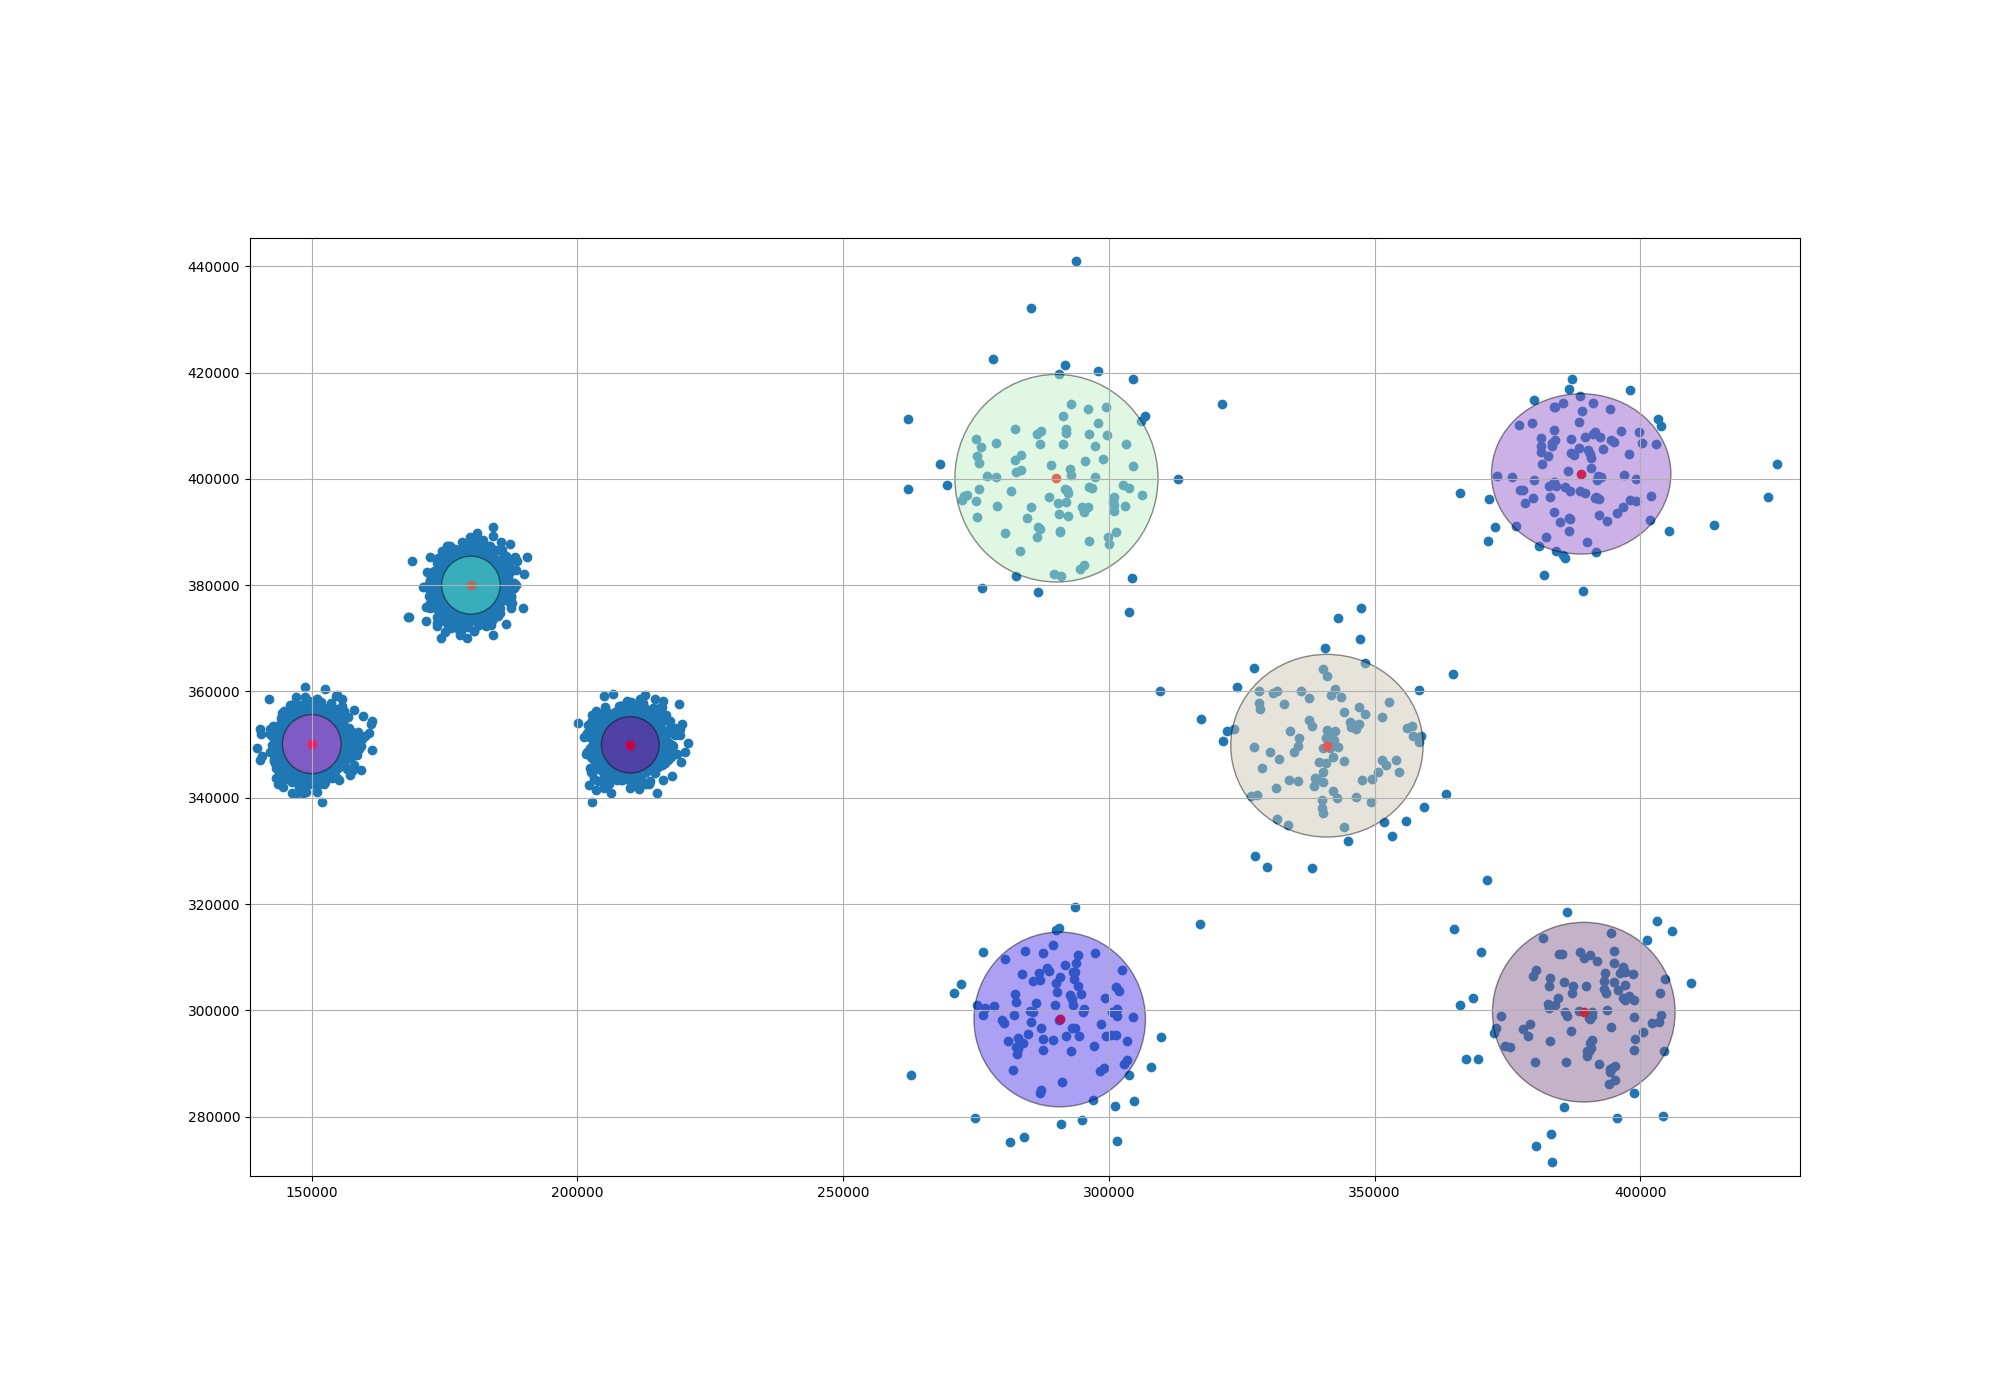
\includegraphics[width=0.5\textwidth]{unbalance_rescaled_density_6.png}}
  \caption{The final outcome of the algorithm.}
  \label{end}
\end{figure}

A noteworthy aspect is that all the aforementioned factors used inside Equation \ref{ellipse_params} have
been set after several tuning stages through empirical tests using many datasets with different
cluster properties.

Nevertheless, representing the clusters my means of sufficient statistics allows to implement an $O(1)$
merging procedure. More in detail, every cluster is internally represented as a touple with the
following imformation:
\begin{equation*}
    \left(\left[\sum_{p}^{|C|} feat[0],\dots,\sum_{p}^{|C|} feat[n]\right],|C|\right)
\end{equation*}
In an 2-dimensional euclidean space, this metadata result in a list containing the the sum of all the
points' coordinates among the 2 axes and the number of points within the cluster taken into consideration.
This structure contains the least possible information to compute the centroid's coordinates as the
barycenter of that particolar cluster.  

Finally, this merging strategy enables all the \emph{Data Mining Desiderata} described in Section 
\ref{intro}. It makes use of sufficient statistics to internally represent the clusters, thus 
requiring an overall amount of memory that is linear in the number of peaks ($O(k)$, \emph{limited memory}
property). Furthermore, the \emph{online} behaviour is guaranteed by default, since the centroid
bootstrap and merging procedure always returns a solution at any point in time. Finally, it allows
to deal with \emph{straming} data thanks both to its linear memory consumption and to its ability to
work with chunks of data by default, propagating all the sufficient statistics needed to update the 
centroids from one iteration to another. This also guarantees that if the computation is stopped
it can restart without having to re-process everything from scratch.


\subsection*{Applications}
The solutions presented in this work can have two main applications. On the one hand,
this procedure can be used as a bootstrapping phase for a  "k-means"-like algorithm. 
On the other, it can be integrated with other partitional clustering algorithms to
refine the local solution every certain number of iterations, allowing the system as a
whole to find increasingly better clusters.